\begin{comment}

% researches suggest\cite{drotar2016evaluation, drotar2015decision, rosenblum2013handwriting}, that handwriting and drawing might serve as a diagnostic biomarker for PD. 

% Main goal of our work is to detect and analyze drawing mistakes within Luria’s alternating series tests of drawing patterns \cite{luria1995higher}, distinguish most significant features, build classification machine learning model and offer mechanism to interpret each individual prediction.

\end{comment}

\section{Motivation}

Gymnastics, a sports discipline with an extensive history, requires athletes to have a comprehensive set of physical traits to execute exercises. These traits include balance, strength, flexibility, agility, and endurance. By developing these physical attributes, the athletes can perform motions involving aerial twisting and rotations. This master's thesis focuses on what is known as \textit{tumbling}, a sub-discipline of gymnastics. Some of the foundation movements in tumbling, ofter categorized as flips and handsprings, include backflips (aka. a back tuck) and back handsprings. These movements form the backbone of tumbling as they are needed to progress onto more advanced moves, while also used as individual components of a tumbling routine.

As backflips and back handsprings are the foundational movements for more advanced exercises, athletes train them regularly. Athlete's perfect their technique until these movements become almost intuitive for a gymnastics athlete. Seasoned athletes experience these exercises' intriguing physical properties, such as the impulse, inertia, rotation, and optimal takeoff angle, without consciously thinking about them. For example, kinematic analysis of the backflip in a tumbling series was conducted on beginner and advanced set of athletes to differentiate their techniques \cite{Burgess2001KINEMATICAO}. The differences in technique between beginner and advanced athletes contribute to both competition score and injury risk, so optimal technique can be considered a priority for every athlete.

At the time of writing, the most common methods for analyzing gymnastics movements require sophisticated motion capture tools, physically attached sensor data, and gymnastics coaches' attention to give valuable feedback to the athletes or analyze their technique \cite{park2014kinematic} \cite{yamada2019dynamics}. This master's thesis focuses on the automatic recognition of backflips and back handsprings using a combination of pose estimation tools with recurrent neural networks. The author proposes the single-camera solution presented in this thesis as a non-invasive, accessible, and state-of-the-art solution to recognize backflips and back handsprings. While not part of this thesis, the author also hopes to contribute the solution developed in this thesis to future research in automated analysis of technique, feedback for athletes, and automatic documentation of gymnastics workouts' history.

\section{Human Activity Recognition Background}

Human activity recognition taxonomy can be challenging as the diversity of available methods is extensive. We depict the broad categorization of human activity recognition methods in figure \ref{har-taxonomy}, proposed in the article \cite{10.3389/frobt.2015.00028}. We also categorize the technique used to automate gymnastics activity recognition in this paper as a \textit{unimodal shape-based method}. While identifying gymnastics movements from multiple modalities (i.e., the addition of behavioral or emotional features) could provide useful data for the analysis, it would require more invasive tools, such as microphones and physical sensors. The author aims to develop a recognition method less invasive and free of physical attachments. For example, in competition environments, athletes are not allowed to wear any extra accessories \cite{acrobatic-gymnastics-rules-and-policies}, and the only viable method for recording the activity is the video modality. 

Narrowing down on unimodal methods and considering the non-invasiveness of shape-based methods, brings the author to a technique called \textit{pose estimation}, a popular research topic in the last ten years. More recently, computationally effective 2D pose estimation methods in real-time using Part Affinity Fields have been proposed \cite{DBLP:journals/corr/CaoSWS16}. This method is also used by the OpenPose software \cite{DBLP:journals/corr/abs-1812-08008}, which is the choice of pose estimation software in this research. 

\begin{figure}[htb]
  \centering
    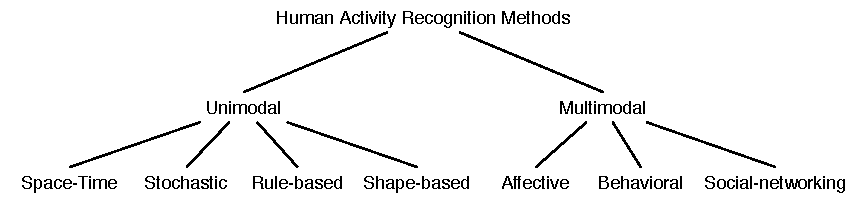
\includegraphics[width=\textwidth,keepaspectratio]
    {images/introduction/har-taxonomy.pdf}
    \caption{Hierarchical categorization of human activity recognition methods}
    \label{har-taxonomy}
\end{figure}

% tendency showing movement in direction of different tests digitized versions



% extend previous research by introducing novel method of drawing pattern analysis 

% Distinction from others
% - luria patterns are rarely used
% - existing studies only analyze whole pattern or strokes
% - logical structure of the pattern is not being taken into account
% - new clustering solution, relatively positioned and sized pattern elements
% - pattern transformation into tree-like graph structures
% - interpretable clusters complimented with parameters
% - anomaly detection 

% Thesis organized as follows
% - 
% - 
% - 


% Main focus of present thesis is to analyze Luria’s drawing patterns of tested individuals, extract interpretable features and produce machine learning model, capable of correct differentiation between groups of healthy controls and Parkinson’s disease patients.

% Luria’s alternating series fine motor tests are being used in psychology and neurology to assess level of disorder in motion planning and execution during handwriting, which is approved biomarker for Parkinson’s disease diagnosis.

% A novel method to analyze Luria’s alternating series patterns drawn during fine motor test constitute main result of the present thesis. Majority of solutions available in the literature are based either on the analysis of entire drawing or individual strokes. Distinctive feature of the proposed approach is that it allows to analyze patterns considering their logical structure with any required level of detail. To achieve this, unique supervised and unsupervised machine learning techniques are applied. Computer vision technique is used to split pattern into logical segments. Based on this information, feature sequences describing different kinematic properties of the drawing are constructed. During next stages, neural-network based models are used to generate feature sequences of the "expected" normal drawing, which allows to highlight "unexpected" regions with anomalies.